\section{Software Development Life Cycle}
\label{sec:sdlc}

\ac{SDLC}\index{software development life cycle} is the fundamental process of software development that involves series of steps or phases, ensures the software completion.
Essentially speaking, it is a series of steps that provide a model for a or collection of software development and its lifecycle management.

\begin{figure}[htbp]
    \centering
    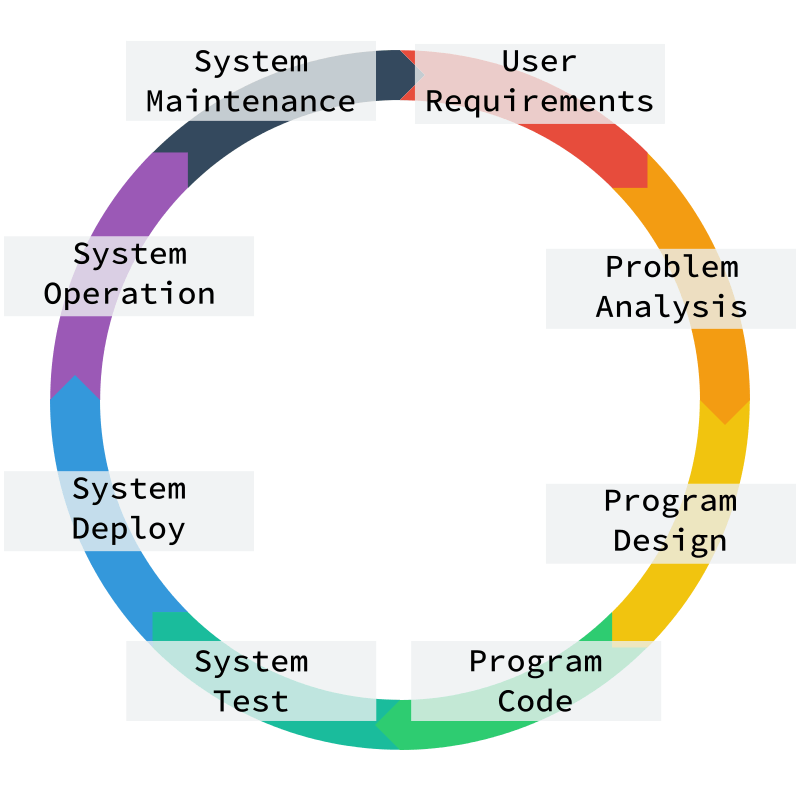
\includegraphics[width=0.8\textwidth]{\dir/include/sdlc.png}
    \caption{Common SDLC Cycle}
    \label{fig:sdlc:cycle}
\end{figure}

As in \autoref{fig:sdlc:cycle}, commonly there are step components like requirements, analysis, design, development (coding), test, deployment, operation, evaluation, and maintenance.
In this kind of traditional \ac{SDLC}, each step should finished its process before go into the next step.

% --------------------------------------------------
\subsection{Agile Methodologies}

Agile is a time boxed, iterative approach to software delivery that builds software incrementally from the start of the project, instead of trying to deliver it all at once near the end.
It works by breaking projects down into little bits of user functionality called user stories, prioritizing them, and then continuously delivering them in short two week cycles called iterations.~\autocite{Rasmusson2015Agile}
\autoref{fig:agile-a} and \autoref{fig:agile-b} shows how agile works in the process and iteration with a simple illustration.

\begin{figure}[htbp]
    \centering
    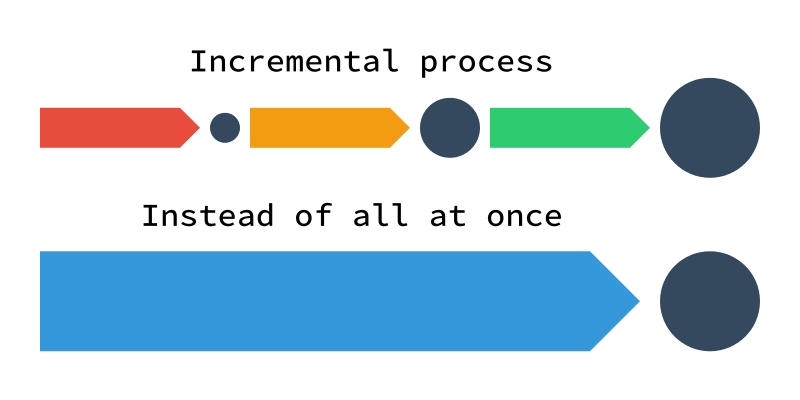
\includegraphics[width=8cm]{\dir/include/agile-a.png}
    \caption{Agile progress}
    \label{fig:agile-a}
\end{figure}

\begin{figure}[htbp]
    \centering
    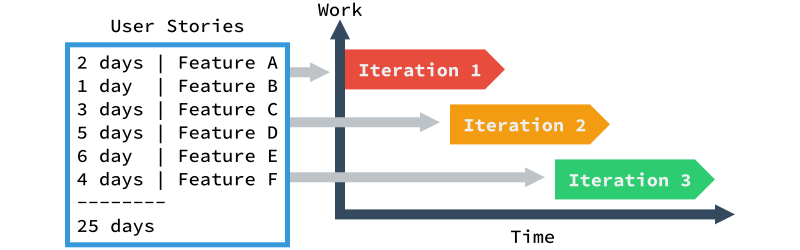
\includegraphics[width=12cm]{\dir/include/agile-b.png}
    \caption{Agile iteration}
    \label{fig:agile-b}
\end{figure}

Therefore, there is no huge risk in creating a big or even a thing that small for a long time.
Because the development can frequently iterate the result, coming back again as like a improved beginning.
Essentially, learn and relearn on what could have done in each iteration process.
In a process matter of sense, analysis, design, development/coding, and testing are continuous activities.
If saw in a traditional perspective, the result of it might look an unfinished thing and the current result may different with the initial requirement.
But the real actualization of agile will be an incremental process and always improving over time, unlike most traditional process that will only have all in one take chance, so that the actions that will be taken is considered still align with the initial purpose.
In addition, there are some key points that required and make agile considered to be greatly modern and fast paced:

\begin{easylist}
& Development itself is iterative
& Planning is adaptive
& The scope variables may vary
& Requirements can change over time
& Working software is the primary measure of success
& Temporary or finished software can be done at all time
& Team members can be independent to each other, since there are cross-functional teams
& High cooperation can occur between technical and non-technical person
& and other leaned segments or aspects to consider
\end{easylist}

Agile is the counterpart of traditional \ac{SDLC}, and it is not just one thing, but a group of methodologies.
As in traditional \ac{SDLC} like waterfall approach, the development cannot change easily any of its parts until it had complete its step.
So if a change is really needed, most likely the entire project will be build from the start again.
Tha means that agile continuous activities are countering traditional approach which has fixed discrete phases.
In agile for example, development can do fix and test at the end of each development step, depending on the corresponding step that matters.
Simply, agile methodologies provide flexibility to make changes, allow for any modification along the progress of \ac{SDLC}.
Hence there could be simultaneous development of different steps at the same time.
But back again, it would depend on the team's or personal's task distribution.
If the conditions are met, agile is more relevant to be used in real modern software development.
Agile method even has a manifesto that offer how convenience agile is, called \textit{Manifesto for Agile Software Development}~\autocite{Beck2001Manifesto}.
The actual circumstances of agile in real world may vary a lot, depending on the team vision and capabilities.
But in common one person or small team operation who use agile for sofware, basically have these steps iterated:
\begin{inparaenum}[\itshape a\upshape)]
\item discover: analyzing and writing initial requirements with acceptance criteria
\item design: sketching, or wireframing, or mocking up
\item development: building, coding, programming, and testing
\item delivery: releasing, deploying, and fixing
\end{inparaenum}
In reality, the condition will be less documentation but more deliverable software that work and viable to user.
Even documentation could rest on all of those steps and naturally created while doing them.
So the time and effort in agile are very directed towards a working thing rather than specifications.
It is a value-driven process rather than plan-driven process.

There are numerous techniques that used when building a software using agile approach.
Some of them are creating user stories and data schema that built using only text explanation, require no diagram or so ever.

For user stories, the explanation format is like ``As a \textit{Subject}, I can \textit{do this}, so that I can \textit{get this}''.
It's also possible to put the required effort points to do so, and place them in the user stories.
From scale the lowest, easiest, or shortest to highest, hardest, or longes may vary but most of the practices use scale in range of $?, 0.5, 1, 2, 3, 5, 8, 13, 21$, which $?$ is still unknown.
These numbers can be in terms of hours or days.
However the implementation can use any other scale like ``quick, easy, medium, hard'' in terms of difficulty.
For example, the user stories are now can be formatted like:

\begin{easylist}[itemize]
& $[1]$ As a \textit{System}, I need to \textit{be something}, so that I can \textit{be something}.
& $[3]$ As a \textit{User}, I can \textit{do something}, so that I can \textit{get benefit}.
\end{easylist}

For data schema, it's like just creating a list like this defining the data or entity name and its attributes.
This way it doesn't require so much time because there is no need to involve graphics and positioning.

\begin{easylist}[itemize]
& Data Name A
  && ID, Date Created, Date Updated, Key Name 1, Key Name 2, ...
& Data Name B
  && ID, Date Created, Date Updated, Key Name 3, Key Name 4, ...
\end{easylist}

% --------------------------------------------------
\subsection{Minimum Viable Product (MVP)}

Agile methodologies also heavily corresponds with building a \ac{MVP}\index{Minimum Viable Product} or can also called a \ac{MWT}\index{Minimum Working Thing}.
Shortly defined, each elements of \ac{MVP} are~\autocite{Montgomery2013MWT}:

\begin{description}
  \item[Minimum] The least or smallest amount possible.
  \item[Viable] Capable of working successfully.
  \item[Product] An article or substance that is created or refined for sale.
\end{description}

Based on those elements, \ac{MVP} is a product that is usable buy ready for the actual and real use.
It establishes incremental steps of usefulness, rather than declare that the product can be useful when it has many features.
Because often the actual needs are just a few things that essentials to the product.
\ac{MVP} can be illustrated as creating a vehicle with two different procedures.
As in \autoref{fig:method:mvp-1}, the first one is a need to take a lot of steps of before finally finished the final usable product.
The second one is an incremental steps of creating the usable product, until it's final yet to be usable as visioned and planned.
It can be seen that the second approach is more appealing and effective than the first.

\begin{figure}[!ht]
    \centering
    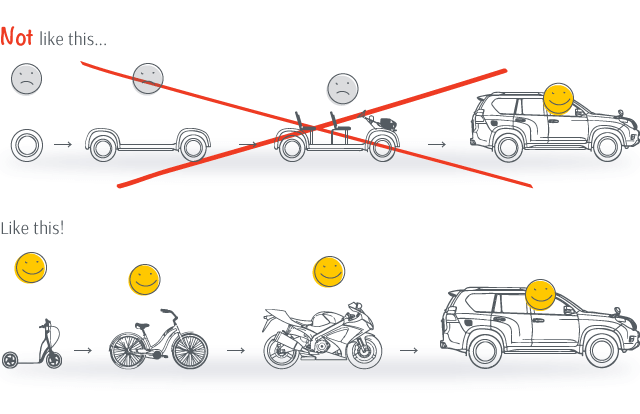
\includegraphics[width=\textwidth]{\dir/include/mvp-1}
    \caption[MVP illustrated]{MVP illustrated with only one usable product and some incremental products~\autocite{Mercury2014MVP}}
    \label{fig:method:mvp-1}
\end{figure}

\begin{figure}[!ht]
    \centering
    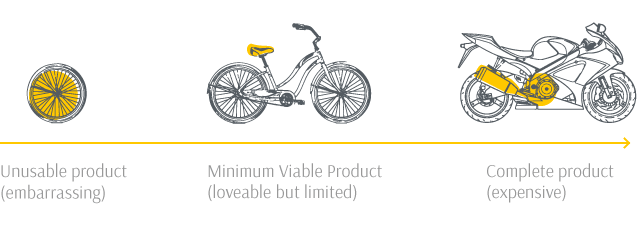
\includegraphics[width=\textwidth]{\dir/include/mvp-2}
    \caption[MVP compared]{MVP compared with unusable and complete product~\autocite{Mercury2014MVP}}
    \label{fig:method:mvp-2}
\end{figure}

Also as in \autoref{fig:method:mvp-2}, \ac{MVP} is compared with unusable product and complete product.
In this context, \ac{MVP} is ideally more balanced and preferable than the others.
More than that, if there is more effort and time, building a \ac{MLP}\index{Minimum Loveable Product} is possible.
Which is an \ac{MVP} but taken beyond a working thing, which the customer will actually love using.
It's an embodiment of a production ready and could potentially get a customer or lots of them.
The thing that matters and can be used well.
Although it expected to be a real matter, such preliminary model like a protoype, a mockup, or even a set of data can sometimes considered as an \ac{MVP}.
